\documentclass[tikz,border=2pt]{standalone}
\usepackage{amsmath}
\usepackage{pgfplots}
\pgfplotsset{compat=1.18}
\usepgfplotslibrary{fillbetween}

\begin{document}
% Uniform convergence: from some n on, the whole graph of f_n lies inside the ε-tube around f
% (the same ε works at every x at once). Here f_n(x) = x^2 + sin(6x)/n.
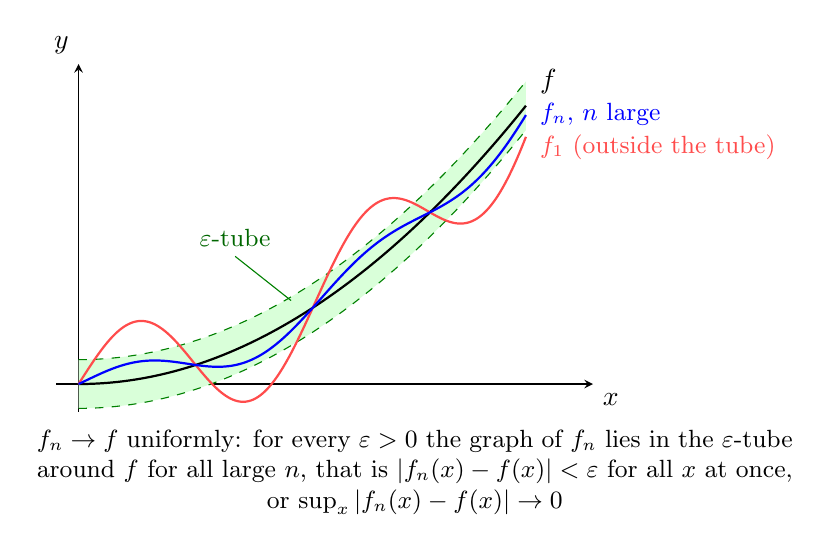
\begin{tikzpicture}
	\begin{axis}[
		axis lines=middle,
		xmin=-0.1, xmax=2.3,
		ymin=-0.4, ymax=4.6,
		xtick=\empty, ytick=\empty,
		xlabel={$x$}, ylabel={$y$},
		xlabel style={below right}, ylabel style={above left},
		samples=250, smooth, clip=false,
		width=8.4cm, height=6cm
		]
		\addplot[name path=upper, draw=none, domain=0:2] {x^2+0.35};
		\addplot[name path=lower, draw=none, domain=0:2] {x^2-0.35};
		\addplot[green!15] fill between[of=upper and lower];
		\addplot[green!50!black, dashed, domain=0:2] {x^2+0.35};
		\addplot[green!50!black, dashed, domain=0:2] {x^2-0.35};
		\addplot[thick, black, domain=0:2] {x^2};
		\addplot[thick, red!70, domain=0:2] {x^2+sin(deg(6*x))/1.2};
		\addplot[thick, blue, domain=0:2] {x^2+sin(deg(6*x))/4};
		\node[black, anchor=west] at (axis cs:2.02,4.35) {$f$};
		\node[red!70, anchor=west, font=\small] at (axis cs:2.02,3.4) {$f_1$ (outside the tube)};
		\node[blue, anchor=west, font=\small] at (axis cs:2.02,3.88) {$f_n$, $n$ large};
		\node[green!40!black, font=\small] (tube) at (axis cs:0.7,2.1) {$\varepsilon$-tube};
		\draw[green!50!black, thin] (tube.south) -- (axis cs:0.95,1.2);
	\end{axis}
	\node[anchor=north, font=\small, align=flush center, text width=9.6cm] at ([yshift=-2pt]current axis.outer south) {$f_n\to f$ uniformly: for every $\varepsilon>0$ the graph of $f_n$ lies in the $\varepsilon$-tube around $f$ for all large $n$, that is $|f_n(x)-f(x)|<\varepsilon$ for all $x$ at once, or $\sup_x|f_n(x)-f(x)|\to0$};
\end{tikzpicture}
\end{document}
